\documentclass{article}
\usepackage[T1]{fontenc}
\usepackage{lmodern}
\usepackage{graphicx}
\usepackage{amsmath,amssymb}
\usepackage[a4paper,margin=2cm]{geometry}
\usepackage[absolute,overlay]{textpos}
\setlength{\TPHorizModule}{1mm}
\setlength{\TPVertModule}{1mm}
\usepackage[indonesian]{babel}
\usepackage{hyperref}
\setlength{\emergencystretch}{2em}
% unit: Halaman 7

\begin{document}

% === Halaman 7 (llm) ===

\begin{center}
\Huge Kriptografi
\end{center}

\vspace{60mm}

\begin{center}
\color{red} Pesan yang dienkripsi dengan kriptografi menimbulkan kecurigaan bagi pengamat. \\
\color{red} Cipherteks dapat dideteksi keberadaannya.
\end{center}

% deskripsi: Ilustrasi konsep kriptografi yang menunjukkan pengirim, penerima, pesan terenkripsi berupa simbol acak (@2*\$#d(*%7*), dan pengamat yang menggunakan kaca pembesar untuk menyelidiki pesan tersebut.
% bbox normalisasi: [0.1870, 0.2130, 0.8140, 0.7430]
\begin{textblock*}{131.67mm}(39.27mm,63.26mm)
\noindent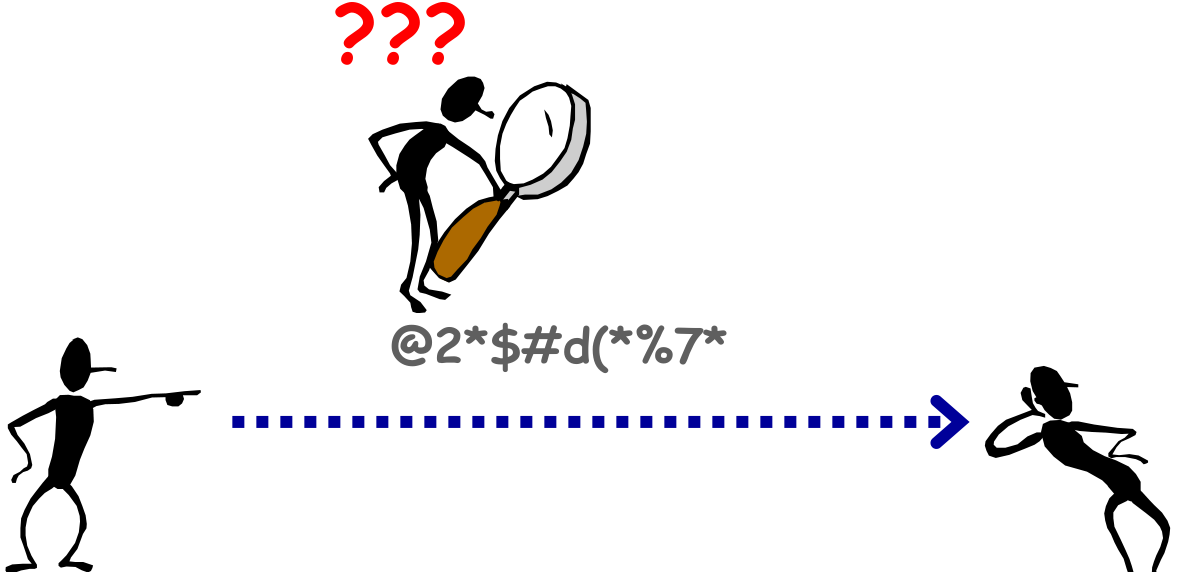
\includegraphics[width=131.67mm,height=157.41mm]{../../images/llm/page_007_img_01.png}%
\end{textblock*}

\end{document}
